%%
% This is an Overleaf template for presentations
% using the TUM Corporate Desing https://www.tum.de/cd
%
% For further details on how to use the template, take a look at our
% GitLab repository and browse through our test documents
% https://gitlab.lrz.de/latex4ei/tum-templates.
%
% The tumbeamer class is based on the beamer class.
% If you need further customization please consult the beamer class guide
% https://ctan.org/pkg/beamer.
% Additional class options are passed down to the base class.
%
% If you encounter any bugs or undesired behaviour, please raise an issue
% in our GitLab repository
% https://gitlab.lrz.de/latex4ei/tum-templates/issues
% and provide a description and minimal working example of your problem.
%%

\documentclass[
  german,            % define the document language (english, german)
  aspectratio=169,    % define the aspect ratio (169, 43)
  % handout=2on1,       % create handout with multiple slides (2on1, 4on1)
  % partpage=false,     % insert page at beginning of parts (true, false)
  % sectionpage=true,   % insert page at beginning of sections (true, false)
]{tumbeamer}

 
% load additional packages
\usepackage{booktabs}
\usepackage{graphicx}
\usepackage{tikz}
\usepackage{url}
\usepackage{pgfplots}
\usepackage{hyperref}
\usepackage{pmboxdraw}
\usepackage{float}
\usepackage{babel}[ngerman]
\usepackage{csquotes}[autostyle]
\usepackage[useregional]{datetime2}
\usepackage{listings}
\usepackage{xurl}
\usepackage{enumerate}
\usepackage{circuitikz}
\usepackage{csquotes}
\usepackage{tikz-timing}
\usepackage{colortbl}

%\usepackage{minted}
%\usemintedstyle{borland}
\usetikzlibrary{patterns}
\pgfplotsset{compat=1.18}

% tikz
\usetikzlibrary{overlay-beamer-styles}
\usetikzlibrary{arrows,backgrounds,positioning,shapes,,patterns,patterns.meta,matrix,arrows,shapes.geometric}
\usetikzlibrary{matrix, fit}
\usetikzlibrary{automata}
% requires circuitikz >= 1.1.0
% for distros with older distributions, install TeX Live manually
% instead of using your package manager
% see: https://tug.org/texlive/quickinstall.html
\ctikzset{logic ports=european}

% minted

\lstset {
    frame=single,
    tabsize=4,
    breaklines=true,
    xleftmargin=5pt,
    xrightmargin=5pt,
    basicstyle=\ttfamily\footnotesize,
    %language=[RISC-V]Assembler,
}

\hypersetup { 
  colorlinks=true,
  urlcolor=blue,
  filecolor=black,
  linkcolor=black
}

% tikz  
\usetikzlibrary{fit}

% image path
\graphicspath{ {../resources/} }

% presentation metadata
\title{Übung 10: Parallelisierung}

\subtitle{Einführung in die Rechnerarchitektur}

\author{\theAuthorName}

\institute{\theGroupName\\\theSchoolName\\\theUniversityName}
\date{06. -- \DTMdisplaydate{2025}{01}{12}{-1}}

\footline{\insertauthor~|~\insertshorttitle~|~\insertshortdate}


% macro to configure the style of the presentation
\TUMbeamersetup{
  title page = TUM tower,         % style of the title page
  part page = TUM toc,            % style of part pages
  section page = TUM toc,         % style of section pages
  content page = TUM more space,  % style of normal content pages
  tower scale = 1.0,              % scaling factor of TUM tower (if used)
  headline = TUM threeliner,      % which variation of headline to use
  footline = TUM default,         % which variation of footline to use
  % configure on which pages headlines and footlines should be printed
  headline on = {title page},
  footline on = {every page, title page=false},
}


% available frame styles for title page, part page, and section page:
% TUM default, TUM tower, TUM centered,
% TUM blue default, TUM blue tower, TUM blue centered,
% TUM shaded default, TUM shaded tower, TUM shaded centered,
% TUM flags
%
% additional frame styles for part page and section page:
% TUM toc
%
% available frame styles for content pages:
% TUM default, TUM more space
%
% available headline options:
% TUM empty, TUM oneliner, TUM twoliner, TUM threeliner, TUM logothreeliner
%
% available footline options:
% TUM empty, TUM default, TUM infoline

\begin{document}

\maketitle

\begin{frame}[c]{Mitschriften \& Infos}{}
  \begin{minipage}[t]{\textwidth}
    \begin{columns}[c]
      \begin{column}{0.8\textwidth}
        Montags: \href{\zulipMo}{\zulipMo}
      \end{column}
      \begin{column}{0.2\textwidth}
        \includegraphics[width=0.8\linewidth]{\zulipMoQrFilename}
      \end{column}
    \end{columns}
  \end{minipage}
  \rule{\textwidth}{0.4pt}
  \begin{minipage}[t]{\textwidth}
    \begin{columns}[c]
      \begin{column}{0.8\textwidth}
        Donnerstags: \href{\zulipDo}{\zulipDo}
      \end{column}
      \begin{column}{0.2\textwidth}
        \includegraphics[width=0.8\linewidth]{\zulipDoQrFilename}
      \end{column}
    \end{columns}
  \end{minipage}
  \ifdefined\myWebsite
  \rule{\textwidth}{0.4pt}
  \centering
  Website: \href{\myWebsite}{\myWebsite}
  \fi
\end{frame}

\begin{frame}[c]{}{}
  \begin{center}
    \LARGE  Keine Garantie für die Richtigkeit der Tutorfolien.

    \Large Bei Unklarheiten/Unstimmigkeiten haben VL/ZÜ-Folien recht!
  \end{center}
\end{frame}

\begin{frame}[c]{Inhaltsübersicht}{}
  \begin{columns}[c]
    \begin{column}{1\textwidth}
      \begin{itemize}
        \item Quiz
        \item Wiederholung
        \item Tutorblatt
        \begin{itemize}
          \item Speedup
          \item Roofline Modell
          \item Auswertung von Speedupdiagrammen
        \end{itemize}
      \end{itemize}
    \end{column}
  \end{columns}
\end{frame}

\begin{frame}[c, fragile]{Parallelisierungstechniken}{}
	\begin{columns}[c]
		\begin{column}{0.5\textwidth}
			\begin{itemize}
				\item Single-Threaded Rechenleistung immer weiter durch physikalische Limits eingeschränkt
				\item Optimierungen: Pipelining, Out-of-Order-Processing, Ausnutzen von Parallelität
				\item SIMD: Eine Instruktion, die gleichzeitig auf mehrere Daten ausgeführt wird (mehr dazu in GRA)

			\end{itemize}
		\end{column}
		\begin{column}{0.5\textwidth}
			\begin{center}
				\resizebox{0.9\textwidth}{!}{
					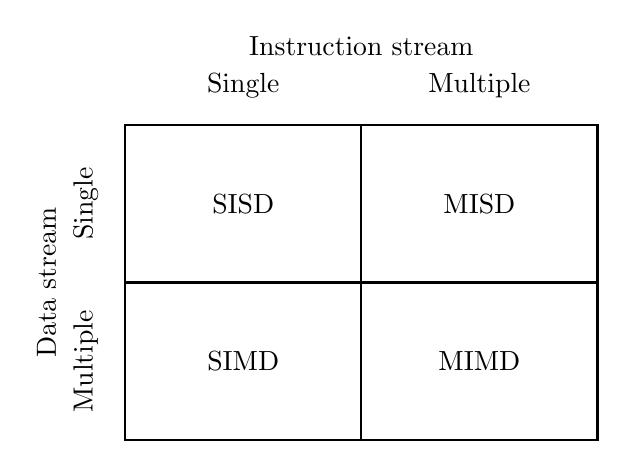
\begin{tikzpicture}[font=\rmfamily]
						\draw[thick] (0,0) rectangle (6,4);

						\draw[thick] (3,0) -- (3,4);
						\draw[thick] (0,2) -- (6,2);

						\node at (1.5,3) {SISD};
						\node at (4.5,3) {MISD};
						\node at (1.5,1) {SIMD};
						\node at (4.5,1) {MIMD};

						\node[rotate=90] at (-0.5,3) {Single};
						\node[rotate=90] at (-0.5,1) {Multiple};
						\node[rotate=90] at (-1,2) {Data stream};

						\node at (1.5,4.5) {Single};
						\node at (4.5,4.5) {Multiple};
						\node at (3,5) {Instruction stream};
					\end{tikzpicture}
				}
			\end{center}
			\centering
			\tiny{Quelle: \href{https://www.researchgate.net/publication/26639095_A_Taxonomy_of_Reconfigurable_Single-Multiprocessor_Systems-on-Chip}{A Taxonomy of Reconfigurable Single-/Multiprocessor\\Systems-on-Chip}}
		\end{column}
	\end{columns}
\end{frame}

\begin{frame}[c, fragile]{MSI/MESI}{}
	\begin{columns}[c]
		\begin{column}{0.5\textwidth}
			\begin{itemize}
				\item Mehrkernsysteme: Was wenn CPU1 und CPU2 beide ein Datum gecached haben und es modifizieren?\\$\rightarrow$ Cache-Inkonsistenzen
				\item Einführung von Zuständen für Cachezeilen
				\item CPUs hören jeweils die Zugriffe der anderen Kerne ab (\enquote{Bus Snooping})
				\item \textbf{M}odified, (\textbf{E}xclusive), \textbf{S}hared, \textbf{I}nvalid
				\item Exclusive-Bit ermöglicht kleineren Overhead wenn CPUs auf verschiedenen Cache-Blöcken arbeiten
			\end{itemize}
		\end{column}
		\begin{column}{0.5\textwidth}
			\begin{center}
				\resizebox{!}{0.8\textheight}{
					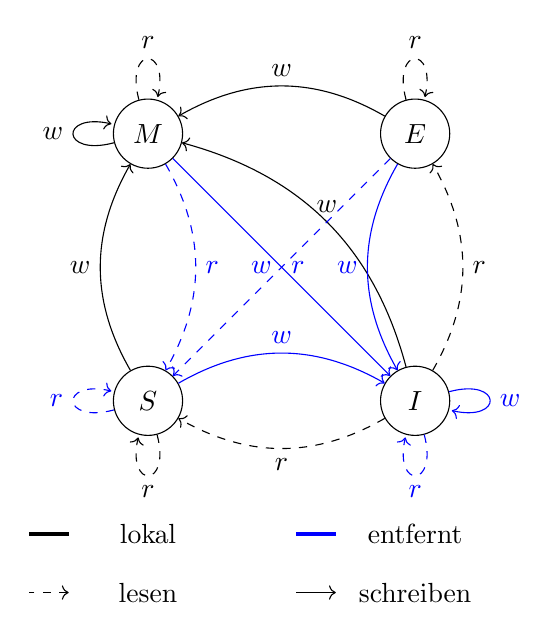
\begin{tikzpicture}
						\tikzset{every node/.style={visible on=<1->},
							label/.style={draw=none},
							local/.style={},
							remote/.style={blue},
							read/.style={dashed,->},
							write/.style={->}
						}

						\def\spacing{2.5cm}
						\def\legSpacing{1cm}

						\node[state] (m) {$M$};
						\node[state] (e) [right=\spacing of m] {$E$};
						\node[state] (s) [below=\spacing of m] {$S$};
						\node[state] (i)  [below=\spacing of e] {$I$};

						% local read
						\path[local, read, visible on=<2->, every node/.style={visible on=<2->, execute at begin node=$, execute at end node=$}]
						(m) edge [loop above] node {r} ()
						(e) edge [loop above] node {r} ()
						(s) edge [loop below] node {r} ()
						(i) edge [bend left, below] node {r} (s)
						(i) edge [bend right, right] node {r} (e);

						% local write
						\path[local, write, visible on=<3->, every node/.style={visible on=<2->, execute at begin node=$, execute at end node=$}]
						(m) edge [loop left] node {w} ()
						(e) edge [bend right, above] node {w} (m)
						(s) edge [bend left, left] node {w} (m)
						(i) edge [bend right, above] node {w} (m);

						% remote read
						\path[remote, read, visible on=<4->, every node/.style={execute at begin node=$, execute at end node=$}]
						(m) edge [bend left, right] node {r} (s)
						(e) edge [right] node {r} (s)
						(s) edge [loop left] node {r} ()
						(i) edge [loop below] node {r} ();

						% remote write
						\path[remote, write, visible on=<5->, every node/.style={execute at begin node=$, execute at end node=$}]
						(m) edge [left] node {w} (i)
						(e) edge [bend right, left] node {w} (i)
						(s) edge [bend left, above] node {w} (i)
						(i) edge [loop right] node {w} ();

						\node[draw=none, minimum width=2cm, below=\legSpacing of s] (leg) {lokal};
						\node[draw=none, minimum width=2cm, below=\legSpacing of i] (leg2) {entfernt};
						\node[draw=none, minimum width=2cm, below=0.25*\legSpacing of leg] (leg3) {lesen};
						\node[draw=none, minimum width=2cm, below=0.25*\legSpacing of leg2] (leg4) {schreiben};


						\draw[very thick, local] (leg.west) -- ++(-0.5,0);
						\draw[very thick, remote](leg2.west) -- ++(-0.5,0);
						\draw[read, <-](leg3.west) -- ++(-0.5,0);
						\draw[, <-](leg4.west) -- ++(-0.5,0);
					\end{tikzpicture}
				}
			\end{center}
		\end{column}
	\end{columns}
\end{frame}


\begin{frame}[c, fragile]{Speedup durch Parallelisierung}{}
	Mit $t_s$ sequentieller Programmteil, $t_p$ paralleler Programmteil, $n$ Anzahl CPU-Kerne,\\$T$ Ausführungszeit mit $n=1$:
	\begin{itemize}
		\item Amdahlsches Gesetz:
		      Gleiche Problemgröße, aufgeteilt auf mehrere Kerne $\rightarrow$ begrenzt durch sequentiellen Anteil
		      \[S_{\textrm{Amdahl}}(n)=\frac{T}{t_s+\frac{t_p}{n}}\]
		\item Gustafsons Gesetz:
		      Mehr Kerne können mehr berechnen: Größeres Problem$\rightarrow$ paralleler Anteil wächst mit Problemgröße, $t_s$ proportional kleiner
		      \[S_{\textrm{Gustafson}}(n)=\frac{t_s+n\cdot t_p}{T}\]
		\item Zwei verschiedene Perspektiven, abhängig von Problemszenario verschieden geeignet
	\end{itemize}
\end{frame}

\begin{frame}[c, fragile]{Amdahlsches Gesetz}{}
	\resizebox{!}{0.8\textheight}{
		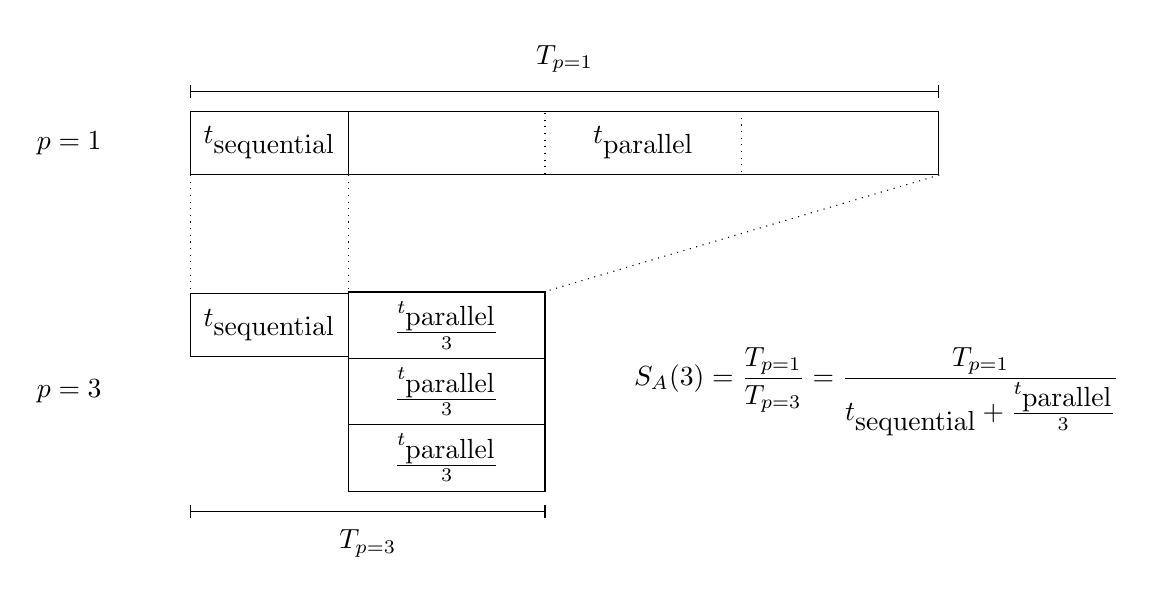
\begin{tikzpicture}
			\tikzset{every node/.style={draw, minimum height=0.8cm, execute at begin node=$, execute at end node=$},
				label/.style={draw=none},
				mapping/.style={dotted}
			}

			\def\seqWidth{2cm}
			\def\parWidth{2.5cm}
			\def\gap{-\pgflinewidth}
			\def\measSpacing{0.25cm}
			\def\compSpacing{1.5cm}

			\onslide<1->{
				\node[minimum width=\seqWidth] (seq1) {t_{\textrm{sequential}}};
				\node[minimum width=3*\parWidth, right=\gap of seq1] (par_comb) {t_{\textrm{parallel}}};
			}

			\onslide<3->{
				\node[minimum width=\parWidth, right=\gap+\parWidth of seq1, dotted] (par_shadow) {};
				%\node[minimum width=\parWidth, right=\gap of par_shadow_2, dotted] (par_shadow_3) {};	
			}

			\onslide<2->{
				\node[minimum width=\seqWidth, below=\compSpacing of seq1] (seq2) {t_{\textrm{sequential}}};
				\draw[mapping] (seq1.south west) -- (seq2.north west);
				\draw[mapping] (seq1.south east) -- (seq2.north east);
			}
			\onslide<4->{
				\node[minimum width=\parWidth, right=\gap of seq2] (par1) {t_{\textrm{parallel}}\over 3};
				\node[minimum width=\parWidth, below=\gap of par1] (par2) {t_{\textrm{parallel}}\over 3};
				\node[minimum width=\parWidth, below=\gap of par2] (par3) {t_{\textrm{parallel}}\over 3};


				%\draw[mapping] (par_shadow.south west) -- (par1.north east);
				%\draw[mapping] (par_shadow.south east) -- (par1.north east);
				\draw[mapping] (par_comb.south east) -- (par1.north east);
			}

			\onslide<5->{
			\draw[{Bar}-{Bar}] ([yshift=-\measSpacing, xshift=-\seqWidth]par3.south west) -- ([yshift=-\measSpacing]par3.south east) node [label, below, midway] {T_{p=3}};
			\draw[{Bar}-{Bar}] ([yshift=\measSpacing]seq1.north west) -- ([yshift=\measSpacing]par_comb.north east) node [label, above, midway] {T_{p=1}};
			}

			\node[label, left=1cm of seq1] {p=1};
			\node[label, left=1cm of par2, xshift=-\seqWidth] {p=3};

			\onslide<6->{
				\node[label, right=of par2] (formula) {\displaystyle S_A(3)=\frac{T_{p=1}}{T_{p=3}} = \frac{T_{p=1}}{t_{\textrm{sequential}}+\frac{t_{\textrm{parallel}}}{3}}};
			}
		\end{tikzpicture}
	}
	\begin{center}
		\tiny{Quelle: Vorlesungsmaterial ERA}
	\end{center}
\end{frame}

\begin{frame}[c, fragile]{Gustafsons Gesetz}{}
	\resizebox{!}{0.8\textheight}{
		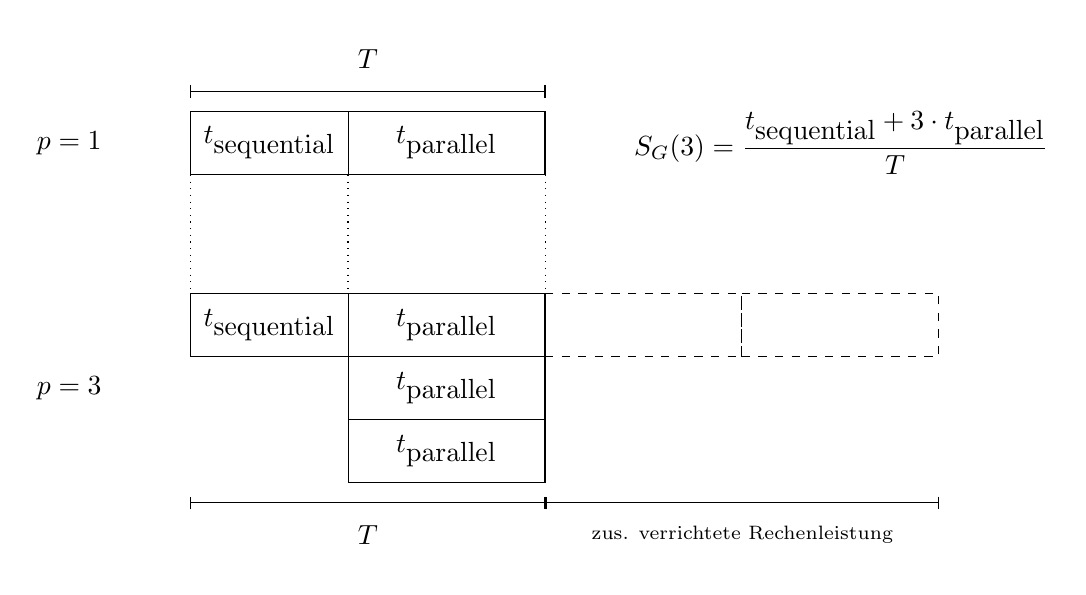
\begin{tikzpicture}
			\tikzset{every node/.style={draw, minimum height=0.8cm, execute at begin node=$, execute at end node=$},
				label/.style={draw=none},
				mapping/.style={dotted}
			}
			\def\seqWidth{2cm}
			\def\parWidth{2.5cm}
			\def\gap{-\pgflinewidth}
			\def\measSpacing{0.25cm}
			\def\compSpacing{1.5cm}

			\onslide<1->{
				\node[minimum width=\seqWidth] (seq1) {t_{\textrm{sequential}}};
				\node[minimum width=\parWidth, right=\gap of seq1] (par_comb)
				{t_{\textrm{parallel}}};
			}

			\onslide<2->{
				\node[minimum width=\seqWidth, below=\compSpacing of seq1] (seq2) {t_{\textrm{sequential}}};

				\node[minimum width=\parWidth, right=\gap of seq2] (par1) {t_{\textrm{parallel}}};

				\draw[mapping] (seq1.south west) -- (seq2.north west);
				\draw[mapping] (seq1.south east) -- (seq2.north east);
				\draw[mapping] (par_comb.south west) -- (par1.north west);
				\draw[mapping] (par_comb.south east) -- (par1.north east);
			}

			\onslide<3->{
				\node[minimum width=\parWidth, below=\gap of par1] (par2) {t_{\textrm{parallel}}};
				\node[minimum width=\parWidth, below=\gap of par2] (par3) {t_{\textrm{parallel}}};
			}

			\onslide<4->{
			\draw[{Bar}-{Bar}] ([yshift=-\measSpacing, xshift=-\seqWidth]par3.south west) -- ([yshift=-\measSpacing]par3.south east) node [label, below, midway] {T};
			\draw[{Bar}-{Bar}] ([yshift=\measSpacing]seq1.north west) -- ([yshift=\measSpacing]par_comb.north east) node [label, above, midway] {T};
			}


			%\draw[mapping] (par2.south east) -- (par_shadow_2.south east);
			%\draw[mapping] (par3.south east) -- (par_shadow_3.south east);

			\onslide<5->{
			\node[minimum width=\parWidth, right=\gap+\parWidth of seq2, dashed] (par_shadow_2) {};
			\node[minimum width=\parWidth, right=\gap of par_shadow_2, dashed] (par_shadow_3) {};

			\draw[{Bar}-{Bar}] ([yshift=-\measSpacing]par3.south east) -- ([yshift=-\measSpacing, xshift=2*\parWidth]par3.south east) node [label, below, midway] {\scriptsize\textrm{zus. verrichtete Rechenleistung}};
			}

			\node[label, left=1cm of seq1] {p=1};
			\node[label, left=1cm of par2, xshift=-\seqWidth] {p=3};

			\onslide<6->{
				\node[label, right=of par_comb] (formula) {\displaystyle S_G(3)= \frac{t_{\textrm{sequential}}+3\cdot t_{\textrm{parallel}}}{T}};
			}
		\end{tikzpicture}
	}
	\begin{center}
	\end{center}
\end{frame}

\begin{frame}[c, fragile]{FLOPS}{}
	\begin{itemize}
		\item Floating Point Operations per Second
		\item Maß für die Leistungsfähigkeit von Computern oder Prozessoren
		\item Beispiele:
		\begin{itemize}
			\item Pentium 4 3,2 GHz: Spitzenleistung 6,4 GFLOPS
			\item Intel Core i7 5820k, 6K/12T, 3,3 GHz: Spitzenleistung 273,1 GFLOPS
		\end{itemize}
	\end{itemize}
\end{frame}

\begin{frame}[c, fragile]{Roofline-Modell}{}
	\begin{columns}[c]
		\begin{column}{0.51\textwidth}
			\begin{itemize}
				\item Modellierung der maximalen Gesamtleistung
				\item X-Achse: Arithmetische Intensität (I)
				\begin{itemize}
					\item in FLOP pro Byte
					\item I = (Anzahl Rechenoperationen in FLOP) / (Speichertransfers in Byte)
					\item Abhängig vom Algorithmus
				\end{itemize}
				\item Y-Achse: Rechenleistung
				\begin{itemize}
					\item in FLOPS
					\item Abhängig vom Rechensystem
				\end{itemize}
				\item Diagonale: Max Speicherbandbreite
				\begin{itemize}
					\item y/x = (GFlop/s) / (Flop/Byte) = GB/s
				\end{itemize}
			\end{itemize}
		\end{column}
		\begin{column}{0.5\textwidth}
			\centering
			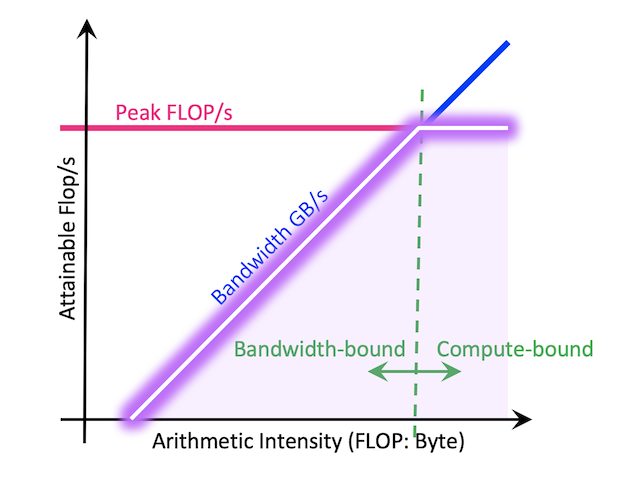
\includegraphics[width=\textwidth]{w10_roofline_google.png}
		\end{column}
	\end{columns}
\end{frame}


\begin{frame}[c]{Feedback}{} 
  \begin{center}
    \includegraphics[width=0.30\textwidth]{\myFeedbackQrFilename}
  \end{center}
  \begin{center}
    \LARGE \href{\myFeedbackLink}{\myFeedbackLink}
  \end{center}
  \vspace{0.5cm}
  \begin{center}
    \small Ein Teil der Folien stammt aus dem Foliensatz von Niklas Ladurner. Vielen Dank dafür!
  \end{center}
\end{frame}

\end{document}